\documentclass[conference]{IEEEtran}
\usepackage{cite}
\usepackage{amsmath,amssymb}
\usepackage{graphicx}
\usepackage{booktabs}
\usepackage{url}
\usepackage[T1]{fontenc}
\usepackage{textcomp}
\graphicspath{{../../results/figures/}}
\hyphenation{Bayes-ian}

\begin{document}

\title{Heart Disease Risk Modelling, Phase~2:\\A Regularised Neural Network versus a\\Hand-Specified Bayesian Network}

\author{
\IEEEauthorblockN{Aaryan Yadav}
\IEEEauthorblockA{2401010011\\aaryan.yadav2024@nst.rishihood.edu.in}
\and
\IEEEauthorblockN{Shivam Mishra}
\IEEEauthorblockA{2401010442\\shivam.mishra2024@nst.rishihood.edu.in}
\and
\IEEEauthorblockN{Satyam Kumar}
\IEEEauthorblockA{2401010429\\satyam.kumars2024@nst.rishihood.edu.in}
\and
\IEEEauthorblockN{Himank Kaushik}
\IEEEauthorblockA{2401010187\\himank.kaushik2024@nst.rishihood.edu.in}
\and
\IEEEauthorblockN{Mohammed Yaseen}
\IEEEauthorblockA{2401010281\\mohammed.yaseen2024@nst.rishihood.edu.in}
\\[1ex]
\IEEEauthorblockA{Deep Learning, Project 15 (Phase 2: neural network and comparison)}
}

\maketitle

\begin{abstract}
Phase~1 of this project compared a hand-specified discrete Bayesian network (BN) with Naive Bayes (NB) and classical baselines on the 303-row UCI processed Cleveland data, and found similar ranking but strongly over-confident probabilities from the two Bayesian models. Phase~2 asks whether a model that \emph{learns} feature interactions from continuous inputs closes that gap. We train a regularised multilayer perceptron (MLP) in PyTorch on scaled numeric and one-hot categorical inputs, with dropout, weight decay, a five-seed ensemble, and architecture, regularisation and epoch count chosen by nested cross-validation. On the same 25 stratified splits used in Phase~1, the MLP reaches an out-of-fold ROC AUC of 0.911 (BN 0.896; paired difference $+0.015$, 95\% interval $[-0.001, +0.031]$) but clearly better probabilities: Brier score 0.117 versus 0.139 (difference $-0.022$ $[-0.036, -0.007]$) and calibration slope 1.00 versus 0.49. An MLP given the BN's own binned inputs is equally well calibrated, so the BN's over-confidence is not caused by discretisation. The MLP is indistinguishable from logistic regression on the same inputs, and SHAP dependence plots are close to additive, so we find no evidence that nonlinear interactions matter at this sample size. SHAP explanations of the MLP and exact weight-of-evidence explanations of the BN broadly agree on which findings matter (rank correlation 0.64). This is a prediction exercise, not clinical decision support.
\end{abstract}

\begin{IEEEkeywords}
multilayer perceptron, Bayesian networks, calibration, SHAP, nested cross-validation, heart disease
\end{IEEEkeywords}

%% ------------------------------------------------------------------------------------
\section{Introduction}
The project contrasts two ways of building a probabilistic classifier for heart disease. A Bayesian network writes the dependence structure down from domain knowledge and estimates conditional probability tables (CPDs) from counts; a neural network learns whatever input interactions the data support. The project brief states the expected gap: \emph{a fixed graph and coarse discretisation can miss continuous and nonlinear interactions among age, heart rate, blood pressure and symptoms}.

Phase~1 (separate report) built the BN, NB, logistic regression and a random forest under one leak-free protocol, with a fixed manifest of 25 cross-validation splits. Its main finding was that ranking (AUC 0.90--0.91) hardly differed between models, while calibration did: the BN and NB had calibration slopes near 0.5. Phase~2 adds the deep-learning model and the comparison the brief asks for. We test four hypotheses, each stated so it can fail:
\begin{itemize}
\item \textbf{H1 (ranking):} the MLP ranks patients better than the BN.
\item \textbf{H2 (probabilities):} the MLP produces better-calibrated probabilities than the BN.
\item \textbf{H3 (source of the gap):} the BN's weakness comes from discretisation rather than from its structure.
\item \textbf{H4 (interactions):} the MLP gains over an additive model with identical inputs, i.e.\ nonlinear interactions carry signal.
\end{itemize}
\emph{Scope and safety.} The label is existing angiographic disease in a 1980s research cohort, not future risk. Nothing here is a medical recommendation.

%% ------------------------------------------------------------------------------------
\section{Background and Related Work}
\textbf{Neural networks for tabular data.} A feed-forward network is very flexible, but on small tabular datasets that flexibility is mostly a liability. A systematic review of clinical prediction models found no average performance benefit of machine learning over logistic regression \cite{christodoulou2019}. With 303 rows we therefore expect, at best, small gains, and treat regularisation as essential.

\textbf{Regularisation.} We use dropout \cite{srivastava2014}, decoupled weight decay (AdamW) \cite{loshchilov2019}, early stopping, and averaging several independently initialised networks, which also tends to improve probability estimates. Modern neural networks are frequently over-confident \cite{guo2017}, so calibration has to be measured, not assumed.

\textbf{Honest tuning.} Choosing hyper-parameters on the same folds used for reporting biases performance upwards \cite{varma2006}. We therefore tune the MLP with nested cross-validation.

\textbf{Explanations.} SHAP \cite{lundberg2017} attributes a prediction to input features using Shapley values from cooperative game theory; Kernel SHAP estimates them for any model by weighted regression on feature coalitions. For a BN classifier with fully observed evidence, the posterior log-odds decompose exactly into a parent term plus one log-likelihood ratio per child of the target; Phase~1 implemented this decomposition. Explaining the MLP's \emph{log-odds} with SHAP puts both models on one scale.

\textbf{Evaluation.} We reuse the Phase~1 metrics and tests: ROC AUC, average precision (AP), sensitivity and specificity at 0.5, Brier score, ECE, and calibration slope and intercept \cite{steyerberg2010}, with paired patient-bootstrap intervals and the Nadeau--Bengio corrected resampled $t$-test \cite{nadeau2003}.

%% ------------------------------------------------------------------------------------
\section{Data and Protocol (shared with Phase~1)}
We use only the official \texttt{processed.cleveland.data} file \cite{janosi1989uci}: 303 patients, 13 predictors (5 numeric, 8 categorical), and the binary target $y=\mathbb{1}[\mathrm{num}>0]$ (139 positive, 45.9\%). Six rows have a missing \texttt{ca} or \texttt{thal}.

All models are evaluated on the \textbf{same 25 splits} (stratified 5-fold, 5 repeats, seed 2026). The Phase~2 notebook rebuilds the splits and asserts that they match the saved Phase~1 manifest, then \emph{reloads} the saved Phase~1 out-of-fold (OOF) predictions rather than refitting the classical models; recomputed Phase~1 metrics match the Phase~1 tables to $10^{-10}$. Metrics are computed per repeat on the 303 OOF predictions and averaged; 95\% intervals come from 500 patient-bootstrap resamples shared by all models, so model differences are paired.

%% ------------------------------------------------------------------------------------
\section{The MLP}
\subsection{Inputs}
The MLP uses exactly the Phase~1 logistic-regression preprocessor: numeric variables are median-imputed and standardised; categorical variables are mode-imputed and one-hot encoded over the full UCI state lists, giving 28 input columns. The preprocessor is fitted only on training rows, inside every outer and every inner fold.

\subsection{Architecture and training}
For an input $x\in\mathbb{R}^{28}$ and hidden sizes $h_1,\dots,h_L$,
\begin{equation}
z_\ell=\mathrm{Dropout}_q\!\left(\mathrm{ReLU}(W_\ell z_{\ell-1}+b_\ell)\right),\quad z_0=x,
\end{equation}
and the output is a single logit $f(x)=w^\top z_L+c$ with $\hat p=\sigma(f(x))$. We minimise binary cross-entropy (log loss) with full-batch AdamW (learning rate $3\times10^{-3}$) in PyTorch \cite{paszke2019}. The final predictor averages the logits of five networks trained from different seeds:
\begin{equation}
\hat p(x)=\sigma\!\Big(\tfrac{1}{5}\textstyle\sum_{k=1}^{5} f_k(x)\Big).
\end{equation}
The single-layer network with 16 units has 481 parameters; the two-layer (32, 16) network has 1,473.

\subsection{Nested tuning}
The search space was fixed before any outer result was seen: hidden layers $\in\{(16),(32,16)\}$, weight decay $\in\{10^{-3},10^{-2},10^{-1}\}$, dropout $\in\{0.1,0.3\}$ (12 configurations). Inside each outer training fold (about 242 rows), a stratified 3-fold inner CV trains each configuration for up to 300 epochs and records the inner validation log loss after every epoch. The (configuration, epoch) pair with the lowest mean inner log loss is selected, and the five-seed ensemble is refit on the full outer training fold for that many epochs. Early stopping therefore uses no outer-fold data, and no rows are held back from the final fit. Log loss was chosen as the criterion because the deliverable is a probability. Outer split $s$ uses seed $s$, so every result is reproducible.

\subsection{Ablations}
\textbf{MLP (binned)} receives the one-hot encoding of the exact bins the BN uses (including the age-adjusted peak heart rate), isolating the effect of discretisation (H3). \textbf{MLP without \texttt{ca}/\texttt{thal}} mirrors the Phase~1 ablation that removes two diagnostic work-up variables.

\subsection{Explanations}
For repeat~0, each held-out patient is explained by the fold model that did not see them. Kernel SHAP explains the MLP logit as a function of the 13 \emph{original} variables (preprocessing inside the explained function), with 40 real complete training-fold rows as background and 500 coalition samples. SHAP values plus the base value reproduce the logit to $5\times10^{-7}$. The BN explanation is the Phase~1 exact weight-of-evidence (WoE) decomposition; it requires complete evidence, so comparisons use the 297 complete rows.

%% ------------------------------------------------------------------------------------
\section{Results}
\subsection{Tuning outcome}
A single hidden layer of 16 units was selected in 22 of 25 outer folds (Table~\ref{tab:hp}), with a median of 73 epochs (range 38--98). Weight decay varied between folds, which suggests a flat optimum. The inner CV consistently preferred the smallest network and stopped training early.

\begin{table}[!t]
\caption{MLP configurations chosen by nested CV (25 outer folds)}
\label{tab:hp}
\centering
\footnotesize\setlength{\tabcolsep}{3.5pt}
\begin{tabular}{lcccc}
\toprule
Hidden units & Weight decay & Dropout & Times chosen & Median epochs \\
\midrule
16 & 0.1 & 0.1 & 7 & 71 \\
16 & 0.1 & 0.3 & 6 & 77 \\
16 & 0.001 & 0.3 & 4 & 72 \\
16 & 0.001 & 0.1 & 2 & 61 \\
16 & 0.01 & 0.1 & 2 & 70 \\
32 $\to$ 16 & 0.001 & 0.3 & 2 & 42 \\
16 & 0.01 & 0.3 & 1 & 84 \\
32 $\to$ 16 & 0.01 & 0.3 & 1 & 49 \\
\bottomrule
\end{tabular}

\end{table}

\subsection{Discrimination and probability quality}
Table~\ref{tab:main} and Fig.~\ref{fig:roc} give the main results. The MLP's AUC (0.911) equals logistic regression's and is within 0.015 of every model. Its probabilities are the best calibrated of all models (slope 1.00, intercept $-0.004$, ECE 0.044), with a Brier score (0.117) level with logistic regression and well below the BN (0.139) and NB (0.126).

\begin{table*}[!t]
\caption{Out-of-fold results on the shared 25 splits (Phase~1 rows reloaded from saved predictions). Sensitivity and specificity at threshold 0.5; slope = calibration slope (ideal 1).}
\label{tab:main}
\centering
\small
\begin{tabular}{lcccccccc}
\toprule
Model & ROC AUC [95\% CI] & AP & Sens. & Spec. & Brier [95\% CI] & ECE & Log loss & Slope \\
\midrule
Naive Bayes & 0.908 [0.874, 0.939] & 0.904 & 0.791 & 0.888 & 0.126 [0.096, 0.155] & 0.087 & 0.456 & 0.51 \\
Bayesian net & 0.896 [0.861, 0.927] & 0.882 & 0.778 & 0.851 & 0.139 [0.107, 0.167] & 0.086 & 0.494 & 0.49 \\
LogReg (binned) & 0.907 [0.870, 0.938] & 0.898 & 0.809 & 0.888 & 0.118 [0.096, 0.144] & 0.050 & 0.380 & 0.99 \\
LogReg (cont.) & 0.911 [0.875, 0.941] & 0.905 & 0.804 & 0.889 & 0.116 [0.094, 0.141] & 0.047 & 0.373 & 0.98 \\
Random forest & 0.908 [0.869, 0.938] & 0.901 & 0.787 & 0.855 & 0.125 [0.106, 0.146] & 0.055 & 0.394 & 1.42 \\
\textbf{MLP} & 0.911 [0.876, 0.942] & 0.901 & 0.810 & 0.876 & 0.117 [0.093, 0.141] & 0.044 & 0.375 & 1.00 \\
MLP (binned) & 0.911 [0.875, 0.942] & 0.904 & 0.804 & 0.889 & 0.115 [0.093, 0.139] & 0.044 & 0.373 & 1.07 \\
\bottomrule
\end{tabular}

\end{table*}

\begin{figure}[!t]
\centering
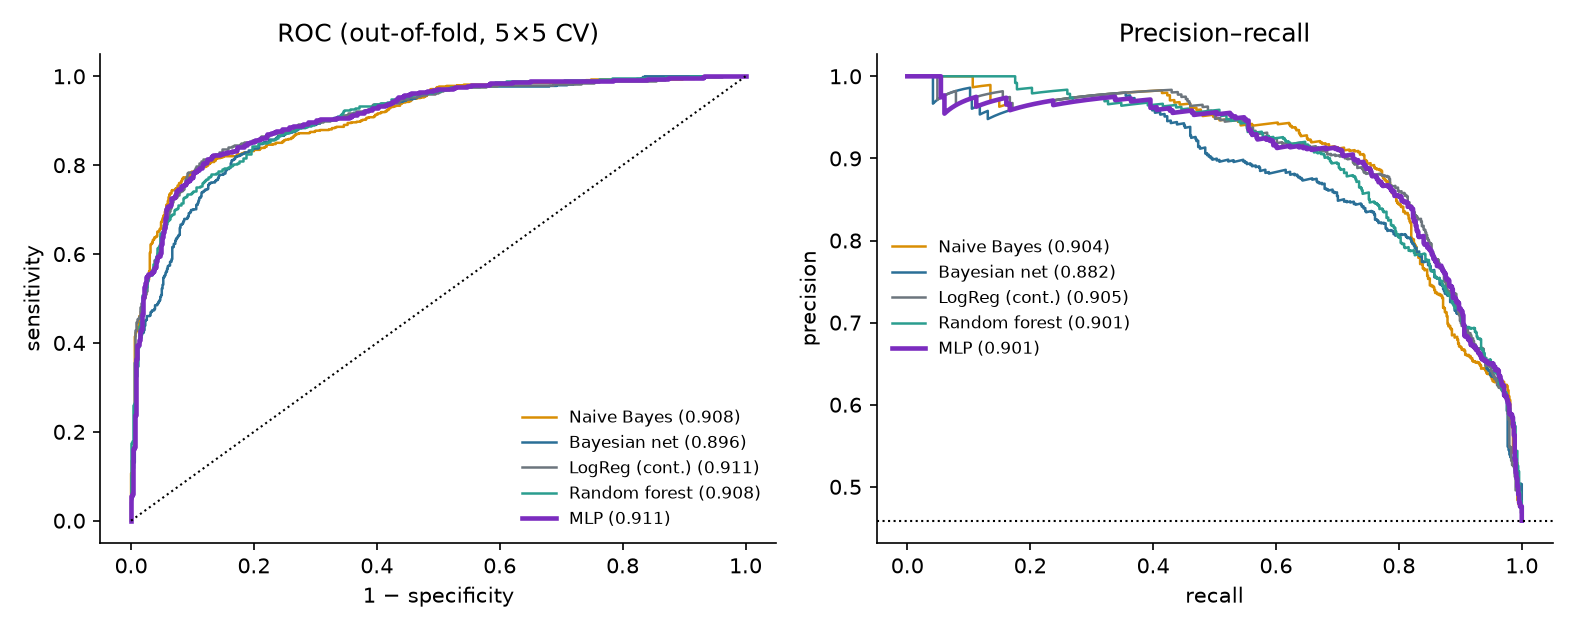
\includegraphics[width=\columnwidth]{fig_p2_roc_pr.png}
\caption{ROC and precision--recall curves, OOF predictions pooled over 5 repeats (descriptive).}
\label{fig:roc}
\end{figure}

\subsection{Calibration}
Fig.~\ref{fig:cal} shows the difference that AUC hides. About 59\% of BN and 64\% of NB OOF predictions lie below 0.05 or above 0.95, versus 30\% for logistic regression and 26\% for the MLP. The BN and NB reliability curves are flatter than the diagonal (over-confident), while the MLP's follows it closely.

\begin{figure*}[!t]
\centering
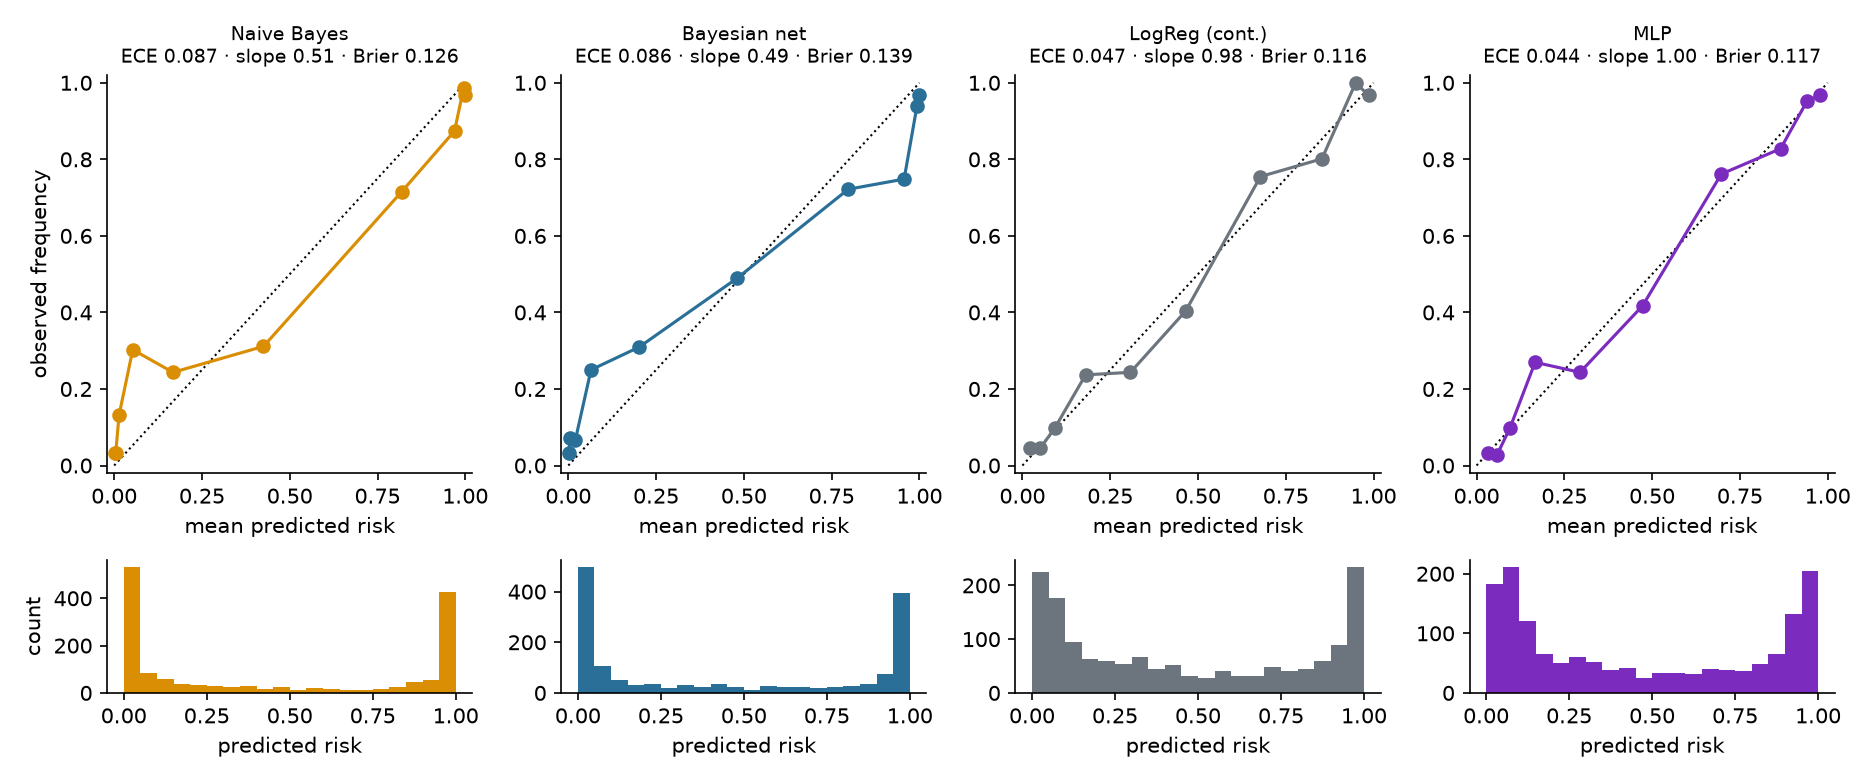
\includegraphics[width=0.9\textwidth]{fig_p2_calibration.png}
\caption{Reliability curves (10 equal-frequency bins, pooled repeats) and histograms of predicted risk.}
\label{fig:cal}
\end{figure*}

\subsection{Paired comparisons}
Table~\ref{tab:paired} lists the exploratory paired comparisons. No AUC difference is detected (all intervals include zero; corrected $p\ge0.11$). Against the BN, the MLP's Brier score is lower with an interval excluding zero, and its AP is higher by a small margin (+0.019 [+0.001, +0.036]). MLP versus logistic regression, with identical inputs, differs by $+0.000$ AUC and $+0.001$ Brier. We stress that a non-significant result does not establish equivalence.

\begin{table*}[!t]
\caption{Exploratory paired comparisons (A $-$ B): paired patient-bootstrap intervals; $p_{\mathrm{corr}}$ is the corrected resampled $t$-test on 25 fold AUCs}
\label{tab:paired}
\centering
\small
\begin{tabular}{lcccc}
\toprule
Comparison (A $-$ B) & $\Delta$AUC [95\% CI] & $p_{\mathrm{corr}}$ & $\Delta$AP [95\% CI] & $\Delta$Brier [95\% CI] \\
\midrule
MLP $-$ Bayesian net & +0.015 [$-$0.001, +0.031] & 0.14 & +0.019 [+0.001, +0.036] & $-$0.022 [$-$0.036, $-$0.007] \\
MLP $-$ Naive Bayes & +0.003 [$-$0.005, +0.014] & 0.41 & $-$0.003 [$-$0.015, +0.010] & $-$0.009 [$-$0.021, +0.001] \\
MLP $-$ LogReg (cont.) & +0.000 [$-$0.005, +0.007] & 0.83 & $-$0.004 [$-$0.010, +0.004] & +0.001 [$-$0.004, +0.005] \\
MLP $-$ Random forest & +0.003 [$-$0.007, +0.015] & 0.47 & $-$0.000 [$-$0.019, +0.018] & $-$0.008 [$-$0.016, +0.001] \\
MLP (binned) $-$ Bayesian net & +0.015 [$-$0.002, +0.030] & 0.11 & +0.021 [+0.005, +0.039] & $-$0.023 [$-$0.036, $-$0.008] \\
MLP $-$ MLP (binned) & +0.000 [$-$0.009, +0.009] & 0.81 & $-$0.003 [$-$0.015, +0.007] & +0.001 [$-$0.005, +0.008] \\
\bottomrule
\end{tabular}

\end{table*}

\subsection{Where does the BN lose? (H3)}
MLP (binned) sees exactly the BN's inputs, yet is calibrated (slope 1.07) and beats the BN on Brier by the same margin as the continuous MLP ($-0.023$ [$-0.036$, $-0.008$]). MLP minus MLP (binned) is $+0.000$ AUC and $+0.001$ Brier. Discretisation therefore cost nothing measurable here, and the BN's over-confidence must come from how evidence is combined: the hand-specified graph treats several correlated findings (exercise angina, ST depression, slope, \texttt{thal}, \texttt{ca}) as conditionally independent given disease, so their likelihood ratios multiply. This is consistent with Phase~1's ESS ablation, where stronger smoothing barely changed the slope. We did not test alternative graphs, so this is an explanation consistent with the evidence rather than a demonstrated cause.

\subsection{Patient-level probability comparison}
Per-patient OOF probabilities of the BN and MLP are strongly rank-correlated (Spearman $\rho=0.94$) and fall on the same side of 0.5 for 92.7\% of patients (Fig.~\ref{fig:pp}). The difference lies in how far the probabilities are pushed: the BN piles patients up near 0 and 1. The BN is confidently wrong ($P>0.9$ for a healthy patient or $P<0.1$ for a diseased one) for 21 patients, the MLP for 5. The largest disagreement is a healthy 51-year-old man with non-anginal pain, no vessels coloured and a normal thallium scan, but with ST depression of 2.4 and a flat ST slope; the BN gives 0.89 and the MLP 0.21.

\begin{figure}[!t]
\centering
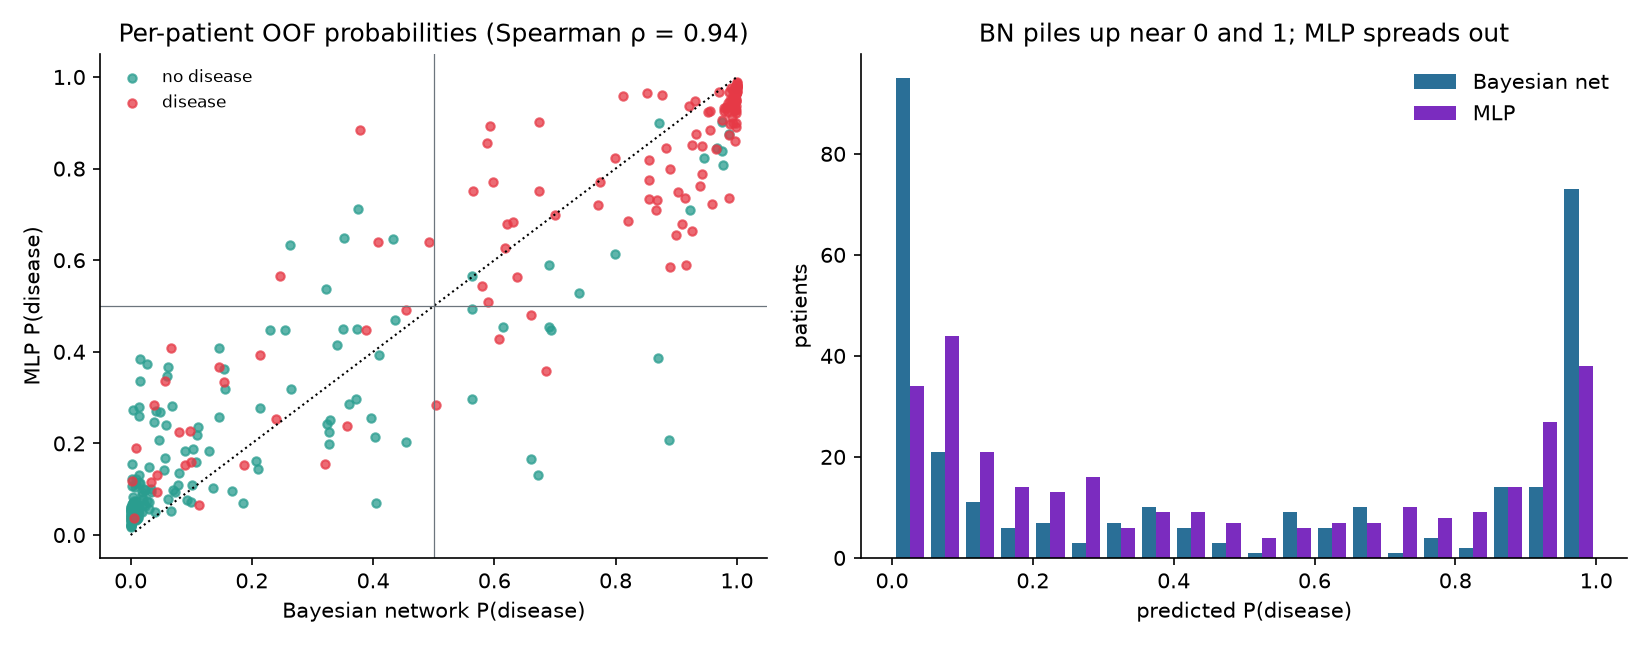
\includegraphics[width=\columnwidth]{fig_p2_bn_vs_mlp.png}
\caption{Left: BN versus MLP probability for every patient (mean over repeats). Right: distribution of predicted probabilities.}
\label{fig:pp}
\end{figure}

\subsection{Explanations: SHAP versus weight of evidence}
Table~\ref{tab:imp} and Fig.~\ref{fig:shap} compare mean absolute contributions on the log-odds scale. Both models rely mostly on \texttt{ca}, \texttt{thal}, chest-pain type and the exercise findings. The rank correlation over the eight shared findings is 0.64. Two differences stand out. First, BN contributions are roughly twice as large, which is the over-confidence seen from inside the model. Second, among risk factors the MLP relies mainly on sex (mean $|$SHAP$|$ 0.36) and blood pressure (0.18), and very little on age (0.06) or cholesterol (0.07).

Fig.~\ref{fig:two} shows the two patients highlighted in Phase~1. Both models agree on direction for nearly every finding, but the BN's terms are larger. For the diseased patient, the BN's heart-rate term even points the other way.

\begin{table}[!t]
\caption{Mean $|$contribution$|$ in log-odds, OOF repeat 0, 297 complete rows. $^\dagger$BN: absolute logit of $P(D\mid\text{parents})$; MLP: sum of SHAP for age, sex, BP, chol, FBS. Not directly comparable.}
\label{tab:imp}
\centering
\footnotesize
\begin{tabular}{lcc}
\toprule
Variable & BN $|$WoE$|$ & MLP $|$SHAP$|$ \\
\midrule
ca & 1.02 & 0.56 \\
cp & 0.81 & 0.56 \\
thal & 1.14 & 0.53 \\
risk factors$^\dagger$ & 1.27 & 0.41 \\
oldpeak & 0.84 & 0.35 \\
heart rate & 0.65 & 0.33 \\
exang & 0.85 & 0.32 \\
slope & 0.49 & 0.30 \\
restecg & 0.35 & 0.15 \\
\bottomrule
\end{tabular}

\end{table}

\begin{figure*}[!t]
\centering
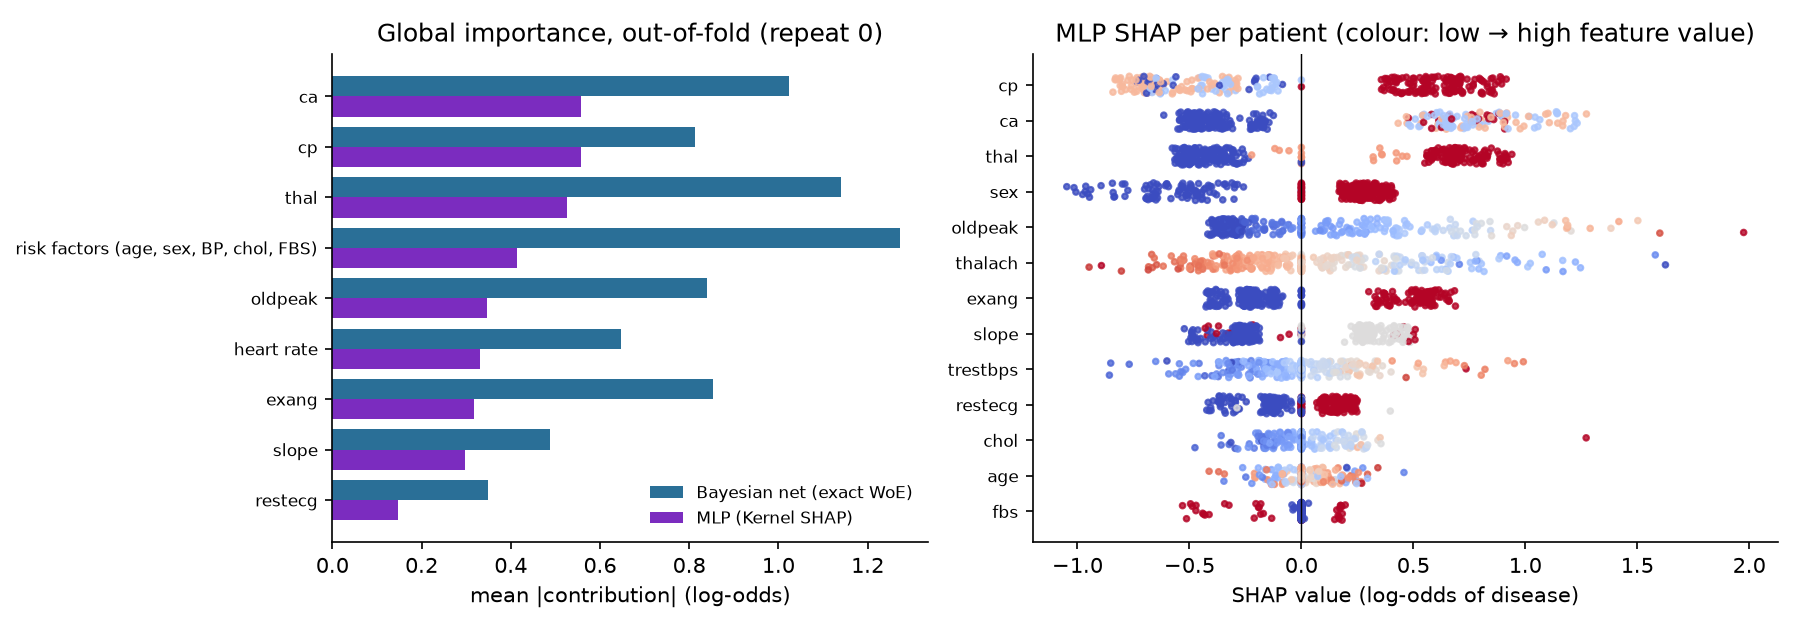
\includegraphics[width=0.92\textwidth]{fig_p2_shap_vs_bn.png}
\caption{Left: global importance, BN exact weight of evidence versus MLP Kernel SHAP. Right: per-patient MLP SHAP values (colour: feature value, low to high).}
\label{fig:shap}
\end{figure*}

\begin{figure*}[!t]
\centering
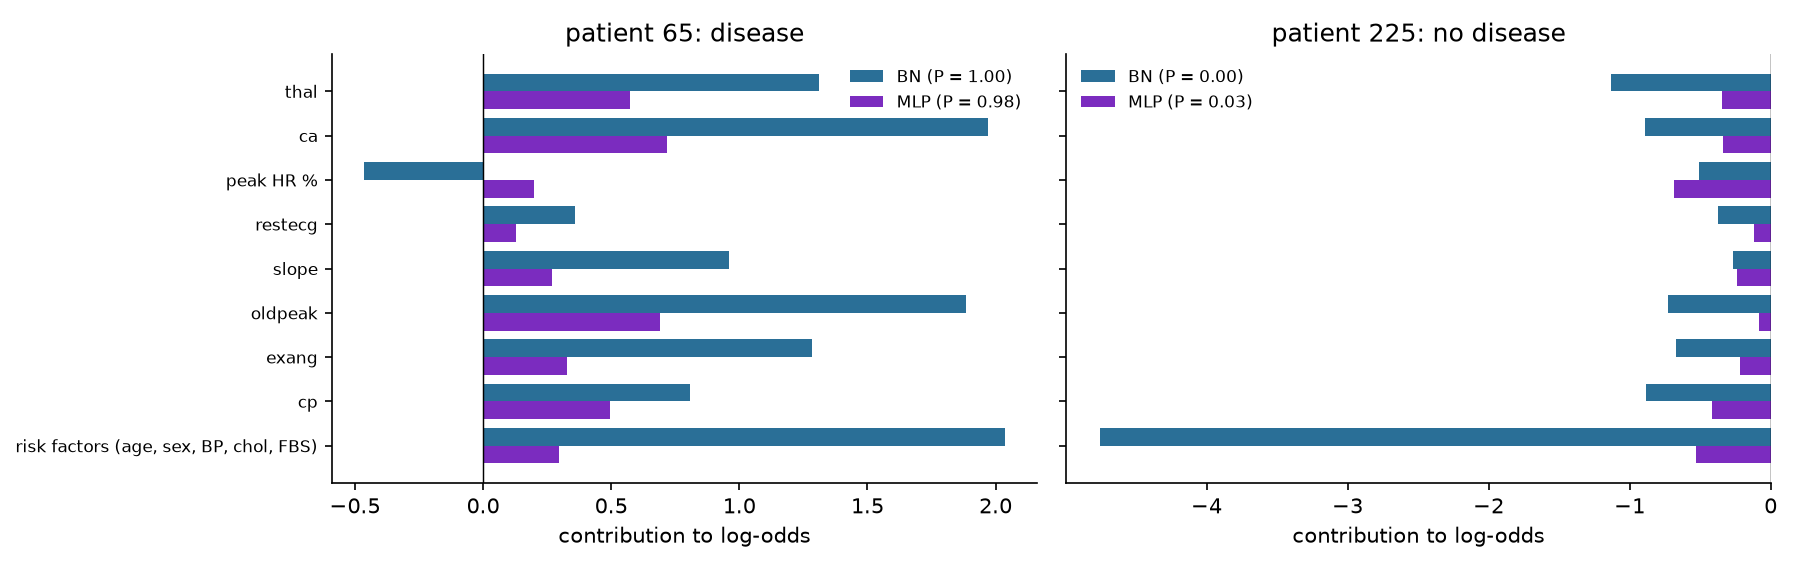
\includegraphics[width=0.85\textwidth]{fig_p2_two_patients.png}
\caption{Two patients explained by both models (log-odds contributions). Contributions describe the models, not causal effects.}
\label{fig:two}
\end{figure*}

\subsection{Interactions (H4)}
If the MLP used interactions, the SHAP value of a variable would vary with \emph{other} variables at a fixed value of its own. Fig.~\ref{fig:dep} shows tight, near-monotone bands. A cubic fit of each variable's SHAP value on its own value explains 98\% of the SHAP variance for ST depression, 93\% for heart rate and 82\% for blood pressure. Age is the exception, but its SHAP values are very small (s.d.\ 0.10). Together with MLP $\approx$ logistic regression and the preference for the smallest network, this indicates the MLP behaves almost additively in the logit.

\begin{figure*}[!t]
\centering
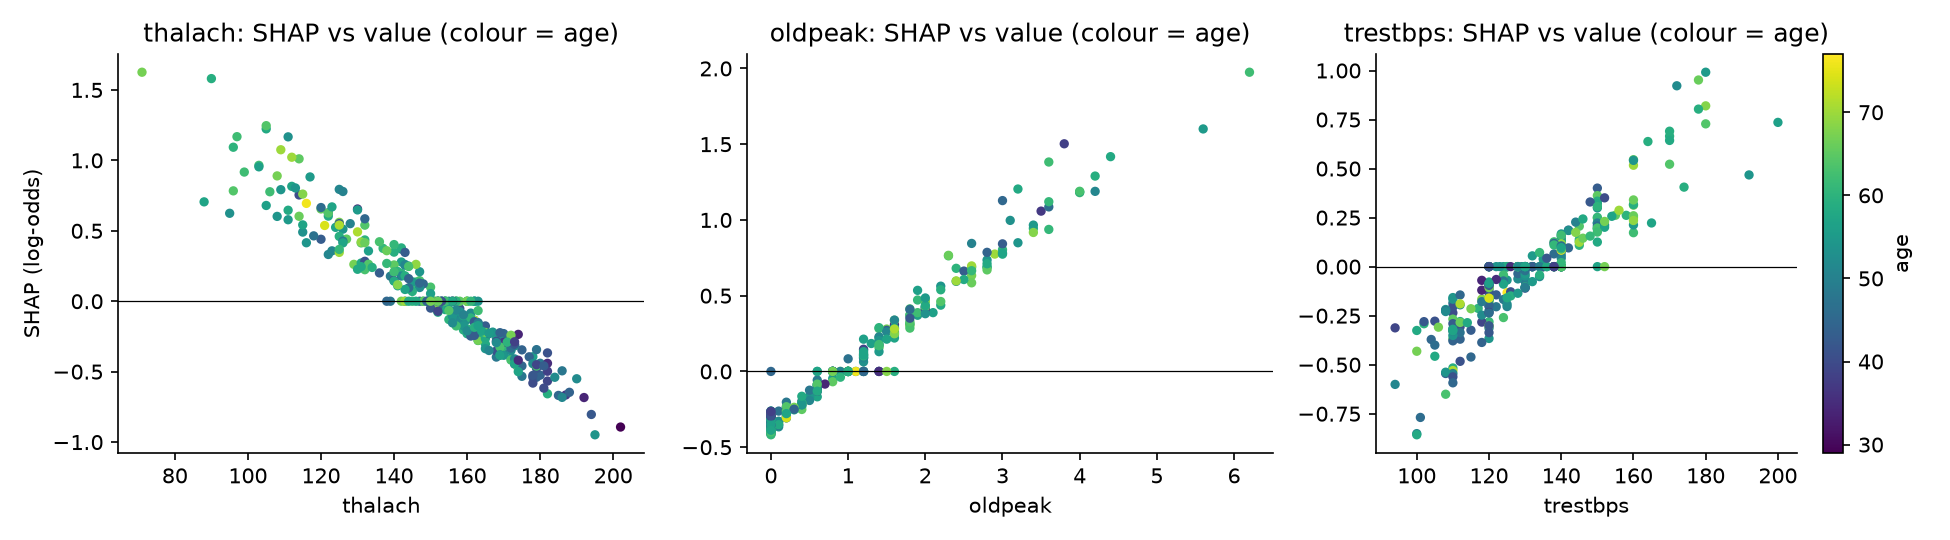
\includegraphics[width=0.85\textwidth]{fig_p2_shap_dependence.png}
\caption{SHAP dependence plots for maximum heart rate, ST depression and resting blood pressure, coloured by age.}
\label{fig:dep}
\end{figure*}

\subsection{Without \texttt{ca} and \texttt{thal}}
Removing the two work-up variables costs every model 0.04--0.05 AUC (Table~\ref{tab:noca}). The MLP (0.868) stays level with logistic regression (0.872) and remains calibrated (slope 0.97), while the BN stays over-confident (0.49). The model-family conclusions do not change.

\begin{table}[!t]
\caption{Models fitted without \texttt{ca} and \texttt{thal} (same 25 splits)}
\label{tab:noca}
\centering
\footnotesize\setlength{\tabcolsep}{3.5pt}
\begin{tabular}{lcccc}
\toprule
Model & AUC [95\% CI] & $\Delta$AUC & Brier & Slope \\
\midrule
Naive Bayes & 0.866 [0.825, 0.906] & $-$0.042 & 0.158 & 0.52 \\
Bayesian net & 0.846 [0.805, 0.884] & $-$0.050 & 0.170 & 0.49 \\
LogReg (cont.) & 0.872 [0.830, 0.909] & $-$0.039 & 0.144 & 0.94 \\
Random forest & 0.862 [0.820, 0.900] & $-$0.046 & 0.151 & 1.21 \\
MLP & 0.868 [0.827, 0.907] & $-$0.043 & 0.146 & 0.97 \\
\bottomrule
\end{tabular}

\end{table}

\subsection{Cost}
A fixed-configuration MLP fit takes about 0.07\,s per fold. Nested tuning (36 inner fits) plus the five-seed refit takes about 2.6\,s, compared with under 0.15\,s for every classical model. The full Phase~2 notebook runs in under five minutes on a laptop CPU.


%% ------------------------------------------------------------------------------------
\section{Discussion}
\textbf{Answers to the hypotheses.} H1 (MLP ranks better than the BN) is \emph{not supported}: the AUC difference is $+0.015$ with an interval that touches zero. H2 (better probabilities) is \emph{supported}: lower Brier score with an interval excluding zero, slope 1.00 versus 0.49, and far fewer confidently wrong predictions. H3 (discretisation causes the gap) is \emph{not supported}: the binned MLP is as good as the continuous one. H4 (interactions carry signal) is \emph{not supported} at this sample size: the MLP matches logistic regression, chose the smallest network, and behaves additively.

\textbf{What the gap really is.} The brief's ``gap'' exists, but not where it was expected. A hand-specified independence structure ranks patients well but multiplies correlated evidence and becomes over-confident. A discriminatively trained model, whether logistic regression or an MLP, learns how much each finding adds \emph{given the others}, and so produces usable probabilities. At $n=303$ the extra flexibility of the MLP neither helps nor hurts: with nested tuning and strong regularisation it collapses to an almost-additive model. This agrees with the tabular and clinical literature \cite{christodoulou2019}.

\textbf{Interpretability trade-off.} The BN offers exact, per-finding explanations and an explicit graph, but its explanations inherit its over-confidence. The MLP needs a post-hoc approximation (SHAP) and a background distribution, but its explanations are on a better-calibrated scale. The two models largely agree on \emph{which} findings matter.

\textbf{Limitations.} 303 historical, single-centre, mostly male rows with no external validation. Patient independence is assumed (no identifiers). The target is existing disease, and \texttt{ca}/\texttt{thal} are work-up results. The 25 splits were already seen in Phase~1, so they are not a fresh test set. The MLP was tuned under nested CV while Phase~1 models used fixed settings; this gives the MLP a fair rather than an unfair budget, but the asymmetry should be noted. Bootstrap intervals condition on fitted predictions and omit training variability. Calibration slope and ECE are noisy at this size. Comparisons are exploratory without multiplicity control, and non-significant differences do not imply equivalence. Kernel SHAP is a sampling approximation that depends on its background and explains model behaviour, not causation. Results can shift slightly across hardware and library versions despite fixed seeds. \textbf{Not for clinical use.}

%% ------------------------------------------------------------------------------------
\section{Reproducibility and Disclosure}
Code, saved splits, OOF predictions, metrics and a 33-test suite are in the project repository. The MLP is in \texttt{src/mlp.py}, SHAP in \texttt{src/explain.py}, and the full analysis in the notebook \path{notebooks/02_phase2_mlp_and_comparison.ipynb}. Every table in this report is generated from \texttt{results/phase2\_*.csv} by \texttt{src/build\_phase2\_tables.py}; no number in a table is typed by hand.

\textbf{Disclosure.} AI tools (Claude, Anthropic) were used to help draft code, analysis and this report; the team is responsible for its contents.

\bibliographystyle{IEEEtran}
\bibliography{references}

\end{document}
